\documentclass[12pt]{standalone}
\usepackage[english]{babel}
\usepackage[utf8]{inputenc}

\usepackage{comment}
\usepackage{amsmath}
\usepackage{tikz}
\usepackage{circuitikz} % for circuits!
\usetikzlibrary{arrows.meta} % for loads
\usepackage{float}
\usetikzlibrary{positioning}
\usetikzlibrary{calc}

\newcommand\ppbb{path picture bounding box}
\tikzset{
  do path picture/.style={%
    path picture={%
      \pgfpointdiff{\pgfpointanchor{\ppbb}{south west}}%
        {\pgfpointanchor{\ppbb}{north east}}%
      \pgfgetlastxy\x\y%
      \tikzset{x=\x/2.5,y=\y/2.5}%
      #1
    }
  },
  sin wave/.style={do path picture={    
    \draw [line cap=round] (-3/4,0)
      sin (-3/8,1/2) cos (0,0) sin (3/8,-1/2) cos (3/4,0);
  }},
	gen/.style={circle, draw=black, thick, minimum width = 2em,sin wave
	},
	cSZ/.style={/tikz/circuitikz/bipoles/length=.6cm}
}


\newcommand{\ctkSZ}{/tikz/circuitikz/bipoles/length=.6cm,}
\newcommand{\csize}{1.5}
\begin{document}
	
	\begin{tikzpicture} [american voltages,scale=.8, 
		breaker/.style={rectangle,draw=black,fill=white},
		load/.style={-{Triangle[length=3.5mm,width=2.5mm,open,fill=black]}},
		node distance = 1.5 cm and 1.5cm]
		
		% Bus Coordinates positions
		% Main Horizontal row
		\node[gen] (G1) at (0,0){};
		\coordinate[right = .5cm of G1](bus1) {};

		\node[gen, below of=G1] (G2) {};
		\coordinate[right = .5cm of G2](bus2) {};
		\coordinate[above right = .5cm of bus2](bus10) {};

		% a = bus number start, b= bus name, c = space between
		\foreach \a/\b/\c in {10/11/\csize, 11/12/\csize,  12/13/\csize*2, 13/14/\csize, 14/15/\csize, }
		\coordinate[right = \c cm of bus\a] (bus\b) {};

		% Vertical draw buses
		\foreach \busNum in {1,2}
		\draw[ultra thick] ([yshift=-0.8cm]bus\busNum.south) -- ([yshift=+0.8cm]bus\busNum.north);

\begin{comment}
		% a = bus number start, b= bus name, c = space between
		\foreach \a/\b/\c in {10/11/\csize, 11/12/\csize,  12/13/\csize*2, 13/14/\csize, 14/15\csize, }
		\coordinate[right = \c cm of bus\a](bus\b) {};
		\node[gen, right =.5 cm of bus3](G3) {};

		% Area Split Line
		\coordinate (areaSplitTop) at at ( $(bus12)!0.5!(bus13)+(0,2)$ ){};
		\coordinate (areaSplitBtm) at at ( $(bus12)!0.5!(bus13)+(0,-4.5)$ ){};
		\draw [dashed] (areaSplitTop) -- (areaSplitBtm);
		\draw ($(areaSplitTop) +(.75,-.2)$) node {\scriptsize{Area 2}}; 
		\draw ($(areaSplitTop) +(-.75,-.2)$) node {\scriptsize{Area 1}}; 
		


		% Second row
		\coordinate (bus2) at ( $(bus6)!0.5!(bus7)+(0,-2.5)$ ){};
		\coordinate (bus5) at ( $(bus10)!0.25!(bus11)+(0,-2.5)$ ){};
		\coordinate (bus4) at ( $(bus3)!0.5!(bus11)+(0,-2.5)$ ){};
		
		\node[gen] (G21) at ($ (-.7 cm,-1.2 cm ) + (bus2)$) {};
		\node[gen] (G22) at ($ (.7,-1.2 ) + (bus2)$) {};
		\node[gen] (G5) at ($ (0,-1.2 ) + (bus5)$) {};
		\node[gen] (G4) at ($ (0,-1.2 ) + (bus4)$) {};
		
		% load coordinates
		\coordinate (load1) at ($ (-.5,-2 ) + (bus8)$) {};
		\coordinate (load2) at ($ (.5,-2 ) + (bus9)$) {};
		
		% Cap coordinates
		\coordinate (cap1) at ($ (+.5,-1.6 ) + (bus8)$) {};
		\coordinate (cap2) at ($ (-.5,-1.6 ) + (bus9)$) {};
		\coordinate (cap3) at ($ (1.2,-1.6 ) + (bus8)$) {};
		\coordinate (cap4) at ($ (-1.2,-1.6 ) + (bus9)$) {};

% caps are scaled, math calcs used for positioning, pretty complicated - could be made simplier by using more defined styles
		\draw ($ (0,-.6) + (bus9)$) -| (cap2) [/tikz/circuitikz/bipoles/length=.6cm, C] to ($(cap2)+(0,-.2)$) node[/tikz/circuitikz/bipoles/length=.7cm,ground] {}; 

		\draw ($ (0,-.6) + (bus8)$) -| (cap1) [/tikz/circuitikz/bipoles/length=.6cm, C] to ($(cap1)+(0,-.2)$) node[/tikz/circuitikz/bipoles/length=.7cm,ground] {}; 

		\draw ($ (0,-.6) + (bus8)$) -- ($ (0,-.6) + (bus8)+(1.2,0)$)  [cSZ, nos] to (cap3) [/tikz/circuitikz/bipoles/length=.6cm, C] to ($(cap3)+(0,-.2)$) node[/tikz/circuitikz/bipoles/length=.7cm,ground] {}; 

		\draw ($ (0,-.6) + (bus9)$) -- ($ (0,-.6) + (bus9)+(-1.2,0)$)  [cSZ, nos] to  (cap4) [/tikz/circuitikz/bipoles/length=.6cm, C] to ($(cap4)+(0,-.2)$) node[/tikz/circuitikz/bipoles/length=.7cm,ground] {}; 
		
		% Vertical draw buses
		\foreach \busNum in {1,6,7,8,9,10,11,3}
		\draw[ultra thick] ([yshift=-0.8cm]bus\busNum.south) -- ([yshift=+0.8cm]bus\busNum.north);
		% Horizontal draw buses
		\foreach \busNum in {5,4}
		\draw[ultra thick] ([xshift=-0.6cm]bus\busNum.west) -- ([xshift=+0.6cm]bus\busNum.east);
		
		% Long Horizontal draw buses
		\foreach \busNum in {2}
		\draw[ultra thick] ([xshift=-1.0cm]bus\busNum.west) -- ([xshift=+1.0cm]bus\busNum.east);

		% xfmrs
		\draw (bus1) to [voosource]  (bus6) {};
		\draw (bus11) to [voosource]  (bus3) {};
		
		\newcommand{\xfmrOff}{.5}
		\draw ($(bus7)+(0,-\xfmrOff)$) -- ($(bus6)!0.5!(bus7)+(0,-\xfmrOff)$) to [voosource] (bus2){};
		\draw ($(bus10)+(0,-\xfmrOff)$) -- ($(bus10)!0.25!(bus11)+(0,-\xfmrOff)$) to [voosource] (bus5){};
		\draw ($(bus11)+(0,-\xfmrOff)$) -- ($(bus3)!0.5!(bus11)+(0,-\xfmrOff)$) to [voosource] (bus4){};
		
		% lines between buses (centered)
		\foreach \a/\b in {6/7,7/8,8/9,9/10,10/11}
		\draw (bus\a) -- (bus\b);
		% lines between gens and buses
		\foreach \a/\b in {1/1,3/3,4/4,5/5}
		\draw (G\a) -- (bus\b);
		% 90 degree lines between gens and buses
		\foreach \a/\b in {21/2,22/2}
		\draw (G\a) |- (bus\b);
		% tripple lines
		\foreach \a/\b in {8/9}{
		\draw ($(bus\a)+(0,-.4)$) -- ($(bus\b)+(0,-.4)$); %
		\draw ($(bus\a)+(0,.4)$) -- ($(bus\b)+(0,.4)$);}
		
		% loads
		% shifting here is of the connection on the bus.
		\draw[load] ($(bus8)+(0,-.6)$) -| (load1) ;
		\draw[load] ($(bus9)+(0,-.6)$) -| (load2) ;
		\draw ($(bus8)+(0,-.6)$) -| (cap1) ;
		
		%bus labels right
		\foreach \busNum in {4,5}
		\draw ($(bus\busNum) +(1,0)$) node {\large{\busNum}};
		%bus labels far right
		\foreach \busNum in {2}
		\draw ($(bus\busNum) +(1.4,0)$) node {\large{\busNum}};
		%bus labels above
		\foreach \busNum in {1,3,6,7,8,9,10,11}
		\draw ($(bus\busNum) +(0,+1.5)$) node {\large{\busNum}};
		
		% gen labels
		\foreach \genNum in{1, 3}
		\draw ($(G\genNum)+ (0,1)$) node (G\genNum){\large G\genNum};
		\foreach \genNum in{4,5}
		\draw ($(G\genNum)+ (1.1,0)$) node (G\genNum){\large G\genNum};
		
		% gen labels on same bus
		\draw ($(G21)+ (-1.6,0)$) node (G21){\large G2 `1'};
		\draw ($(G22)+ (1.6,0)$) node (G22){\large G2 `2'};

\end{comment}
	\end{tikzpicture}
\begin{comment}	
	\begin{tikzpicture} 
	\draw[help lines,step=5mm,gray!20] (-4,-4) grid (4,3);
	\coordinate[draw] (a) at (0,0) {a};  
	\foreach \pos in {above,above right,right,below right,below,below left,left,above left}
	\coordinate[draw,\pos = of a] () {\pos};
	
	\begin{scope}[yshift=8cm,node distance=2cm and 2cm]
	\draw[help lines,step=5mm,gray!20] (-4,-4) grid (4,3);
	
	\coordinate[draw] (a) at (0,0) {a};  
	\foreach \pos in {above,above right,right,below right,below,below left,left,above left}
	\coordinate[draw,\pos = of a] () {\pos};
	\end{scope}
	\end{tikzpicture} 
	
\end{document}


\begin{document}

%3 gen 8 bus
\begin{figure}[H]% system diagram
	\begin{center} 
		% 4 bus, infinite gen power system
		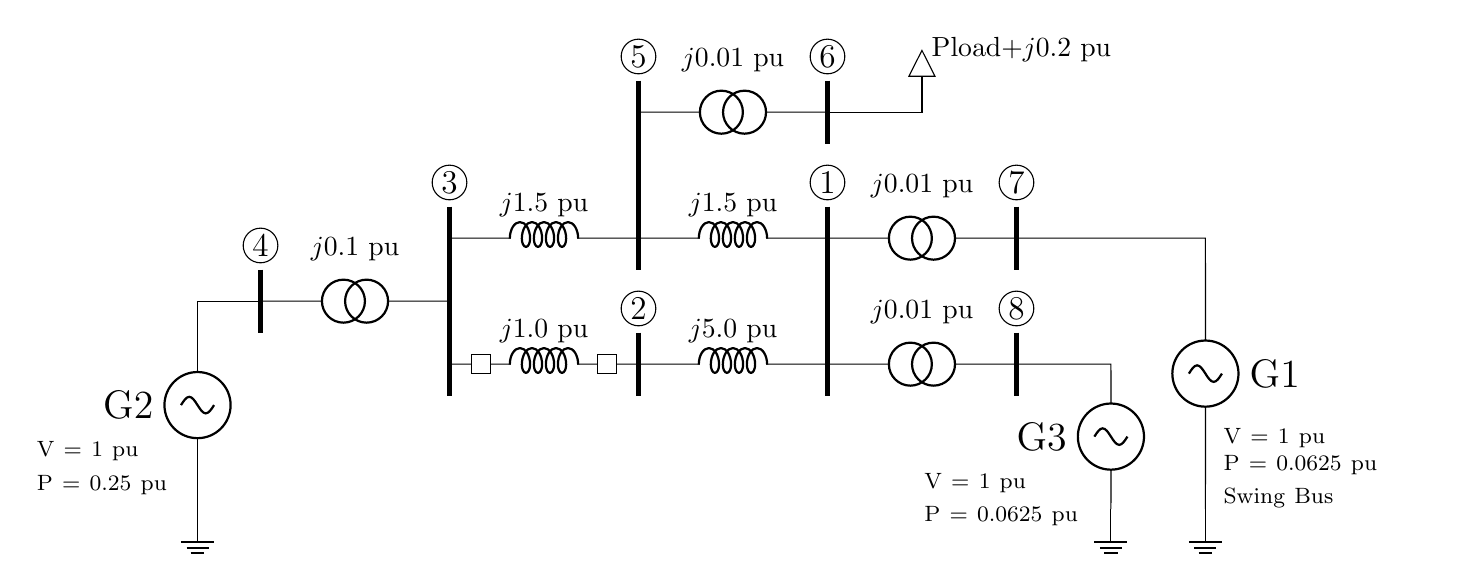
\begin{tikzpicture} [american voltages,scale=.8, 
		breaker/.style={rectangle,draw=black,fill=white}]
		
		% Generators 
		\draw (1,2) to (0,2) to [sV, n=G2] (0,-1.3) node[ground] {}; % G2
		\draw (13,3) to (16,3) to [sV, n=G1] (16,-1.3) node[ground] {}; % g1
		\draw (13,1) to (14.5,1) to [sV, n=G3] (14.5,-1.3) node[ground] {}; % g3
		
		% Labels for gens
		\draw (G2) ++(-1.1,0) node (G2L){\Large G2};
		\draw (G2L) ++(-0.2,-1) node[text width=2cm] {\footnotesize V = 1 pu\\ P = 0.25 pu};
		\draw (G1) ++(1.1,0) node (G1L){\Large G1};
		\draw (G1L) ++(+0.75,-1.5) node[text width=2.5cm] {\footnotesize V = 1 pu\\ P = 0.0625 pu\\Swing Bus};
		\draw (G3) ++(-1.1,0) node (G3L){\Large G3};
		\draw (G3L) ++(-.3,-1) node[text width=2.5cm] {\footnotesize V = 1 pu\\P = 0.0625 pu};
		
		% inductances
		\draw (1,2) to [voosource, l=$j0.1$ pu]  (4,2) {}; % g2 xfmr X
		\draw (4,3) to [L, l=$j1.5$ pu] (7,3); %top branch
		\draw (7,3) to [L, l=$j1.5$ pu] (10,3); %top branch
		\draw (4,1) to [L, l=$j1.0$ pu] (7,1); %lower branch left
		\draw (7,1) to [L, l=$j5.0$ pu] (10,1); %lower branch right
		\draw (7,5) to [voosource, l=$j0.01$ pu] (10,5); %add branch right
		\draw (10,1) to [voosource, l=$j0.01$ pu] (13,1); %xfm to G3
		\draw (10,3) to [voosource, l=$j0.01$ pu] (13,3); %xfm to G1
		
		% Draw Busses - named nodes at top of line
		\draw [ultra thick] (1, 2.5) node (bus4) {} -- (1,1.5) ;	%bus 4
		\draw [ultra thick] (4, 3.5) node (bus3) {} -- (4,.5) ;		%bus 3
		\draw [ultra thick] (7, 1.5) node (bus2) {} -- (7,0.5);	%bus 2
		\draw [ultra thick] (7, 5.5) node (bus5) {} -- (7,2.5);		%bus 5
		\draw [ultra thick] (10, 3.5) node (bus1) {} -- (10,.5) ;	%bus 1
		\draw [ultra thick] (10, 5.5) node (bus6) {} -- (10,4.5) ;	%bus 6
		\draw [ultra thick] (13, 1.5) node (bus8) {} -- (13,0.5) ;	%bus 8
		\draw [ultra thick] (13, 3.5) node (bus7) {} -- (13,2.5) ;	%bus 7
		
		% Labels for busses
		\draw (bus1) ++(0,.1) node[anchor = south,circle,inner sep=1pt,draw] {\large{1}};
		\draw (bus2) ++(0,.1) node[anchor = south,circle,inner sep=1pt,draw] {\large{2}};
		\draw (bus3) ++(0,.1) node[anchor = south,circle,inner sep=1pt,draw] {\large{3}};
		\draw (bus4) ++(0,.1) node[anchor = south,circle,inner sep=1pt,draw] {\large{4}};
		\draw (bus5) ++(0,.1) node[anchor = south,circle,inner sep=1pt,draw] {\large{5}}; 
		\draw (bus6) ++(0,.1) node[anchor = south,circle,inner sep=1pt,draw] {\large{6}};
		\draw (bus7) ++(0,.1) node[anchor = south,circle,inner sep=1pt,draw] {\large{7}};
		\draw (bus8) ++(0,.1) node[anchor = south,circle,inner sep=1pt,draw] {\large{8}};
		% fault location
		%\draw (5.5,0.9) node {\textcolor{m}{\Huge \Lightning}};
		
		% Breakers
		%	\draw (7.5, 5) node [breaker] {};
		%	\draw (9.5, 5) node [breaker] {};
		%	\draw (10.5, 1) node [breaker] {};
		%	\draw (12.5, 1) node [breaker] {};
		\draw (4.5, 1) node [breaker] {};
		\draw (6.5, 1) node [breaker] {};
		
		% loads
		\draw[-{Triangle[length=3.5mm,width=3.5mm,open]}] (10,5)--(11.5,5)--(11.5,6) node[anchor = west] {Pload$+j0.2$ pu};
		%	\draw[-{Triangle[length=3.5mm,width=3.5mm,open]}] (7,-0.5)--(5.5,-0.5)--(5.5,-1.5) node[anchor = east] {$0.325+j0.15$ pu};
		\end{tikzpicture}
		\vspace{-1.5em}
		\caption{100 MVA Power system with generator powers for heavy Pload cases.}
		\label{p_sys}
	\end{center}
\end{figure}

\end{comment}


\end{document}